% !TEX root = ../apprentissage.tex

\section{TIC, éducation et société}

\subsection{Époque ancienne}

\begin{frame}{Antiquité}
\begin{columns}
\begin{column}{0.49\linewidth}
\ldots dans l'éducation
\begin{itemize}
\item Traditions orales
\item Platon~: dialétique
\item épopée comme méthode de mémorisation
\end{itemize}
\end{column}

\begin{column}{0.49\linewidth}
\ldots dans la société
\begin{itemize}
\item écriture
\end{itemize}
\end{column}
\end{columns}
\end{frame}

\begin{frame}{Moyen âge}
\begin{columns}
\begin{column}{0.49\linewidth}
\ldots dans l'éducation
\begin{itemize}
\item moines copistes
\item cours magistraux
\end{itemize}
\end{column}

\begin{column}{0.49\linewidth}
\ldots dans la société
\begin{itemize}
\item imprimerie
\end{itemize}
\end{column}
\end{columns}
\end{frame}

\begin{frame}{Renaissance}
\begin{columns}
\begin{column}{0.49\linewidth}
	\begin{centering}
	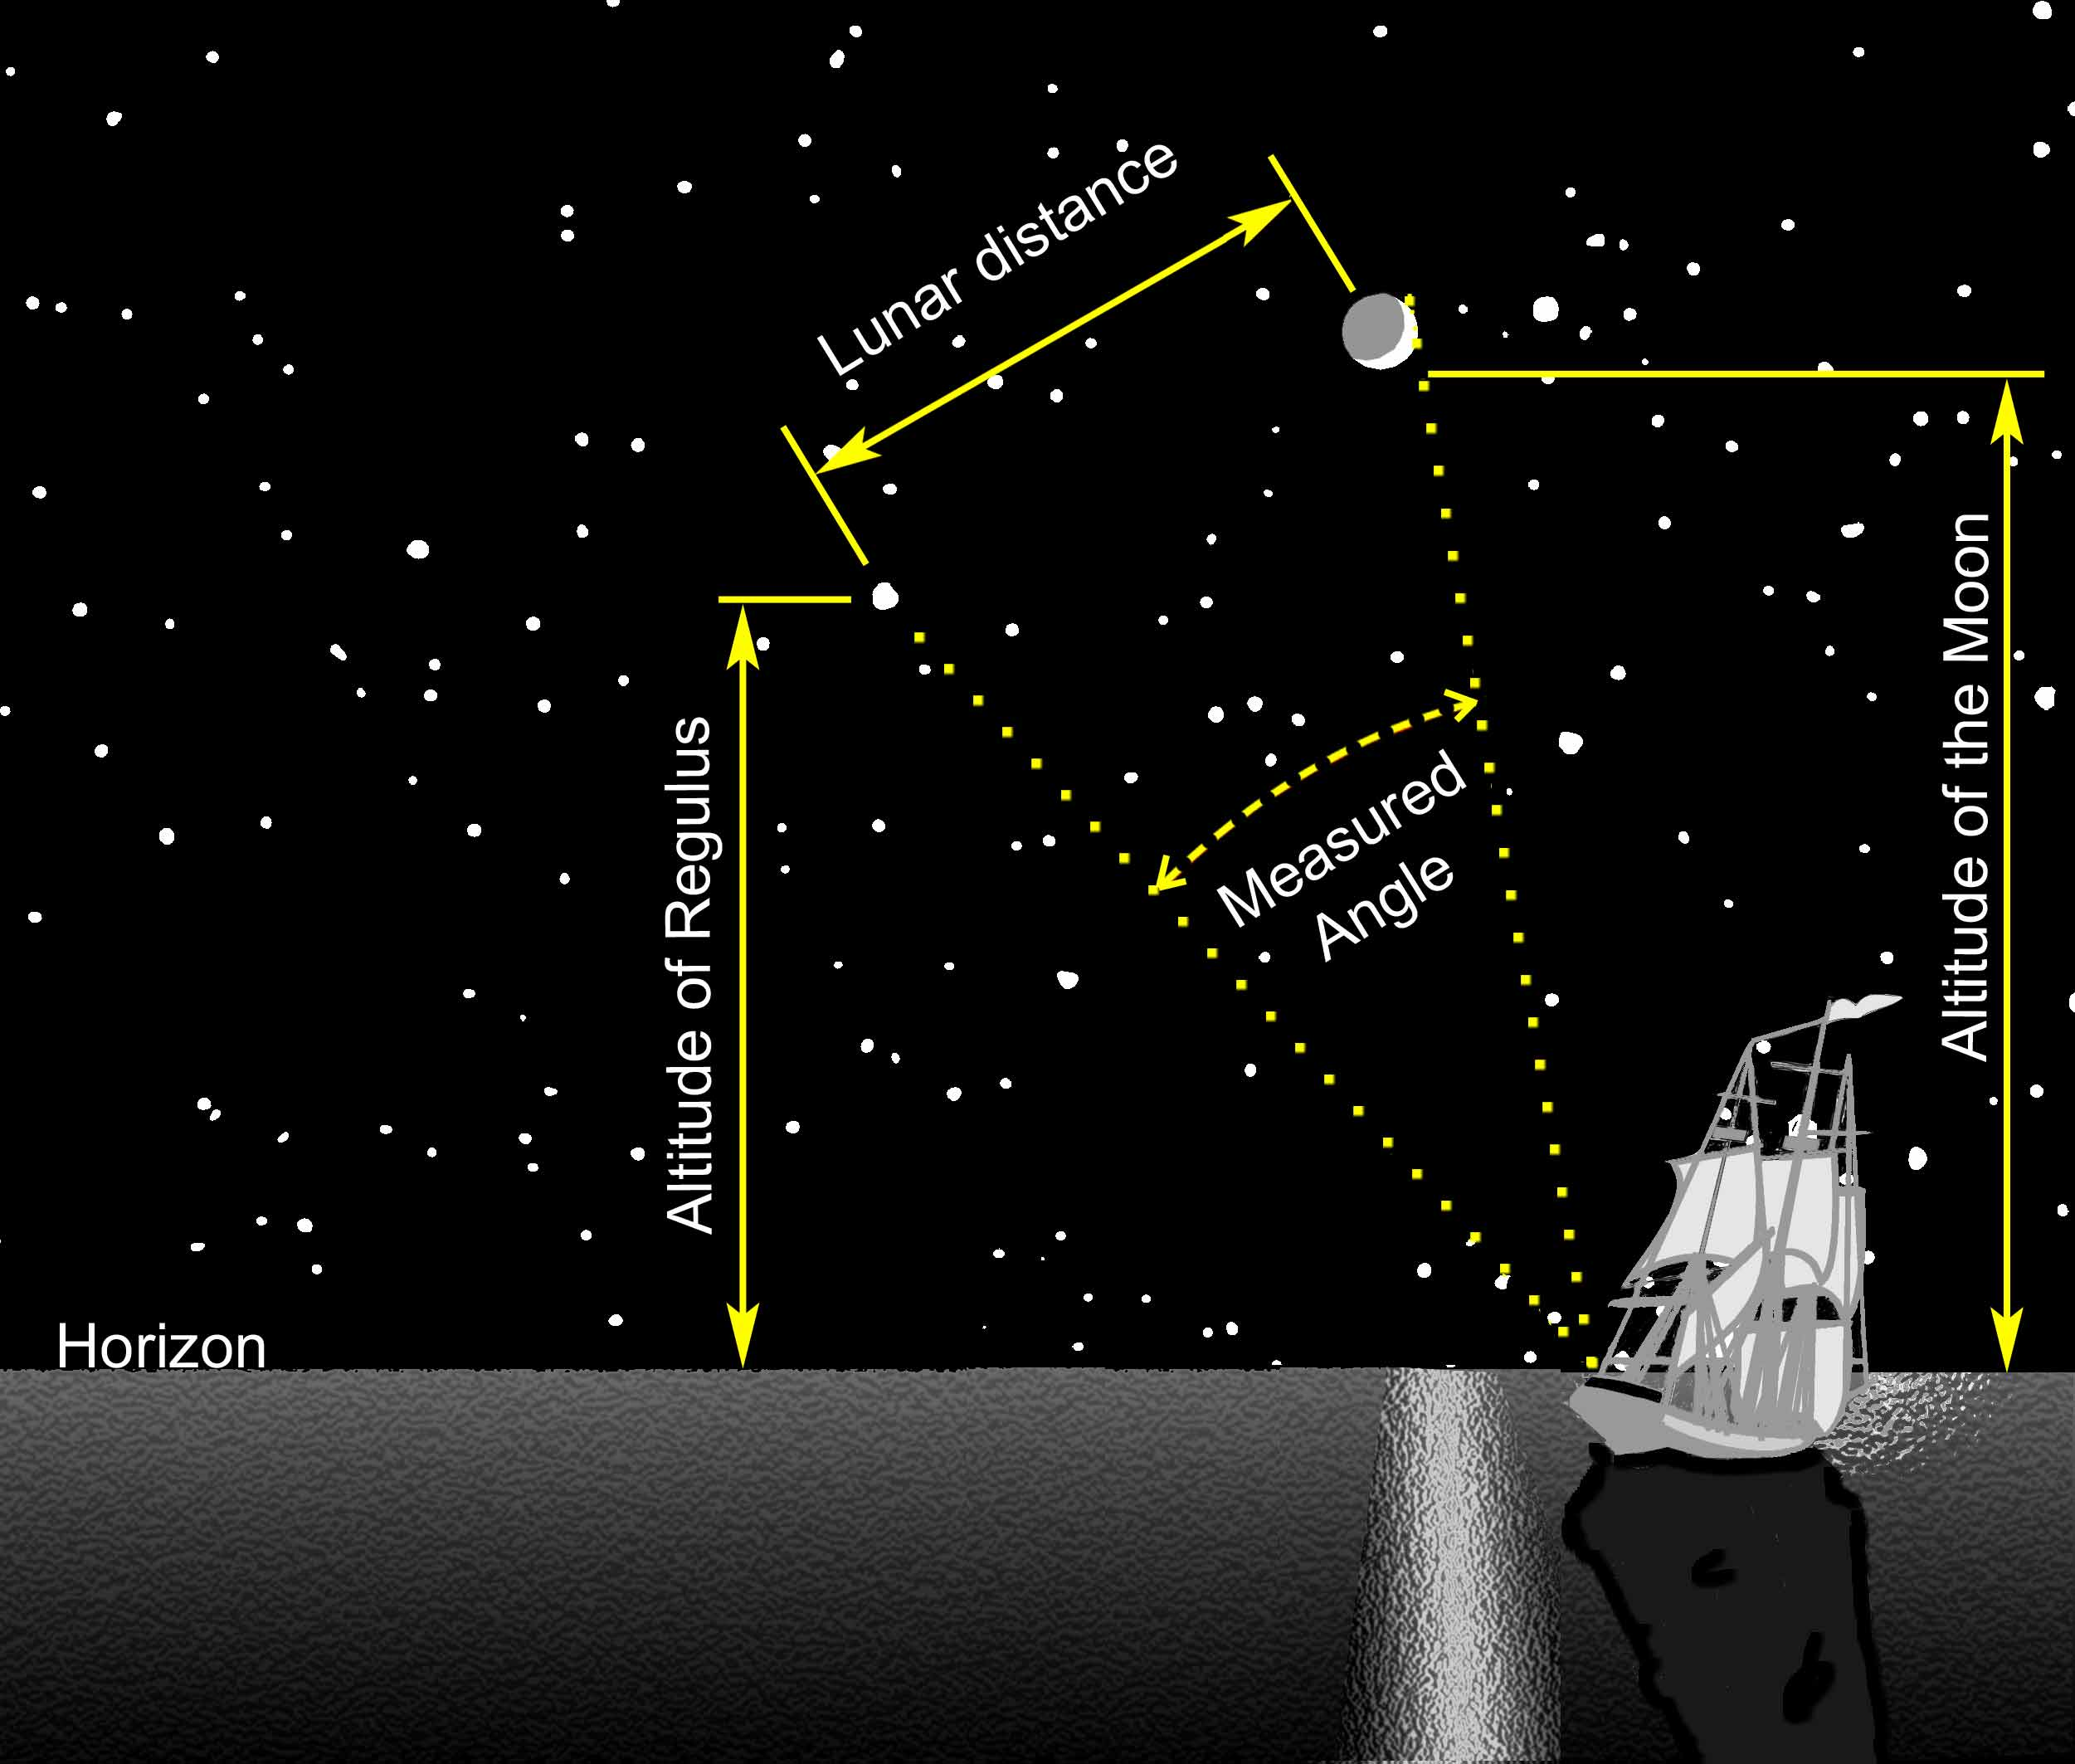
\includegraphics[height=0.4\paperheight]{../resources/illustrations/lunar-distance} \\
	\end{centering}
\ldots dans l'éducation
\begin{itemize}
\item Logarithmes de Neper (1614)
\item Tables, Almanachs
\item Longitude~: distance lunaire
\end{itemize}
\end{column}

\begin{column}{0.49\linewidth}
	\begin{centering}
	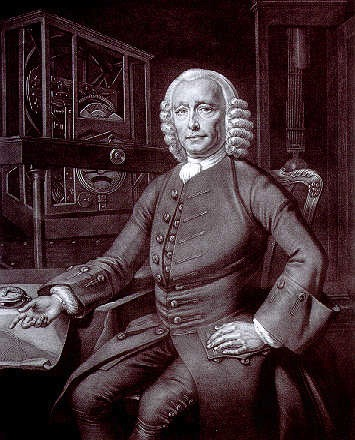
\includegraphics[height=0.4\paperheight]{../resources/illustrations/harrison} \\
	\end{centering}
\ldots dans la société
\begin{itemize}
\item Horloge maritime
\item Mécanisation du calcul
\end{itemize}
\end{column}
\end{columns}
\end{frame}

\subsection{Époque contemporaine}

\begin{frame}{Idée d'une instruction publique}

Révolution française

\begin{quote}
Tant qu'il y aura des hommes qui n'obéiront pas à leur raison seule [\ldots] le genre humain n'en resterait pas moins partagé entre deux classes : celle des hommes qui raisonnent, et celle 
des hommes qui croient.
\end{quote}
Condorcet, avril 1792

\footlineextra{\cite{condorcet_92}}
\end{frame}

\begin{frame}{Bref historique de l'institution scolaire}
\begin{description}
\item[\bf 1833 - loi Guizot] obligeant les communes de plus de 500 habitants à avoir une école primaire de garçons
\item[\bf 1836 - loi Pelet] insitant les communes à avoir une école primaire de filles
\item[\bf 1867 - loi Duruy] obligeant les communes de plus de 500 habitants à avoir une école primaire de filles
\item[\bf 1881 - loi Jules Ferry] établissant la gratuité de l'enseignement primaire
\item[\bf 1882 - loi Jules Ferry] rendant l'école obligatoire pour les enfants de 6 à 13 ans
\end{description}

\footlineextra{\cite{book_serusclat,senat_ferry}}
\end{frame}

\begin{frame}{1881 Bataillon scolaire}
\includegraphicsabsolute{../resources/illustrations/Le-bataillon-scolaire}{.5\textwidth}{1cm}{2cm}
\includegraphicsabsolute{../resources/illustrations/theorie_militaire_zoom}{.4\textwidth}{7cm}{2cm}
\end{frame}

\begin{frame}{test}
  \begin{itemize}
  \item 1890 - Questions pédagogiques, Brouard et Defondon
  \item 1899 - \og{}The child is already intensely active, and the question 
  of eductation is the question of taking hold of his activities, of 
  giving them direction\fg{} John Dewey
  \item 1923 - Constructivisme, Piaget
  \end{itemize}
  
\footlineextra{\cite{book_middle_works_dewey}\cite{piaget_1923}}
\end{frame}


